\documentclass[12pt,a4paper,oneside]{report}
\usepackage[a4paper,margin=1in]{geometry}
\usepackage[T1]{fontenc}
\usepackage[utf8]{inputenc}
\usepackage{lmodern,microtype}
\usepackage{setspace,graphicx,booktabs,tabularx,array,enumitem,hyperref,xcolor,tikz,float,url,listings}
\usetikzlibrary{arrows.meta,positioning,shapes.geometric}
\hypersetup{colorlinks=true,linkcolor=black,citecolor=blue!50!black,urlcolor=blue!50!black}
\setstretch{1.18}
\renewcommand{\arraystretch}{1.15}
\lstset{basicstyle=\ttfamily\footnotesize,breaklines=true,frame=single,columns=fullflexible,showstringspaces=false}
\begin{document}
\begin{titlepage}\centering
\vspace*{0.7cm}
{\Large\bfseries UCS503P -- Project Report\par}
\vspace{1.5cm}
{\Huge\bfseries ResearchAgent: An Autonomous AI Agent for Stock and Company Research\par}
\vspace{0.5cm}{\Large Final Project Report\par}
\vspace{1.5cm}
{\large\bfseries Submitted by\par}\vspace{0.4cm}
Ananya Khanduja, CSED \quad 1024030693\\
Garv Sharma, CSED \quad 1024030695\\
Vishwa Choudhary, CSED \quad 1024030668\\
\vspace{1.2cm}
{\large\bfseries Submitted to\par}\vspace{0.3cm}
{\Large Paramveer Ma'am\par}
\vfill
{\large End-Semester Evaluation\par}
{\large Computer Science and Engineering Department\par}
{\large Thapar Institute of Engineering and Technology, Patiala\par}
\vspace{0.5cm}{\large November 2026\par}
\end{titlepage}

\pagenumbering{roman}
\chapter*{Abstract}
Researching a listed company usually means moving between financial-data portals, news sites, and search engines before a coherent picture emerges. This fragmentation costs time and leads to notes that differ in coverage from one company to the next. ResearchAgent is a web-based, tool-using AI agent that accepts a company name or ticker, gathers evidence through external tools, and writes it up as a structured six-section research brief.

The completed system (version 1.0) has a React 19, Vite, TypeScript, and Tailwind CSS frontend and a Go HTTP API that uses only the Go standard library. The agent follows a Plan--Act--Observe--Reflect--Synthesise loop of at most eight steps, driven by Google Gemini with an optional OpenRouter backup. It dispatches three tools---financial data, news, and web search---each with a layered chain of sources (Twelve Data, Yahoo Finance, Screener.in, Exa, DuckDuckGo, and Google News RSS). Two rules keep the output grounded: the model may not write a report until a tool has returned real data, and when the model is unavailable a deterministic report is built only from retrieved data, with unsupported sections explicitly marked as unavailable.

The final build is verified by 48 Go unit tests and a 15-check HTTP integration script, all passing, and the frontend type-checks and builds from a clean install. A Render deployment Blueprint is included. Runs against live data sources with a real Gemini key, and the proposed timing pilot, could not be carried out in the build environment; time-to-report and grounding quality on live data therefore remain to be measured and are reported as such.

\noindent\textbf{Keywords:} AI agent, company research, tool orchestration, financial information, Go, React, TypeScript.

\tableofcontents
\listoffigures
\listoftables
\clearpage
\pagenumbering{arabic}

\chapter{Introduction}
\section{Background and Context}
Preliminary research on a listed company may involve reviewing financial snapshots, recent news, company and sector context, competitors, and risk factors. These materials are spread across websites that differ in freshness and format. A user has to find relevant sources, cross-check claims, and organise everything into a consistent brief.

Large language models can help with synthesis, but a model-only answer may be out of date or unsupported if it is not grounded in retrieved evidence. A tool-using agent offers a more structured approach: plan research steps, call external tools, inspect their outputs, retry when evidence is missing, and write the report from what was gathered. The engineering challenge is to coordinate tools reliably and to be honest about data that could not be retrieved.

ResearchAgent addresses this with a lightweight web application for students and individual investors. The goal is a dependable research workflow for one company at a time, not new model research or stock-price prediction.

\subsection{Problem Statement}
The project proposal~\cite{proposal} identified four pain points:
\begin{itemize}[leftmargin=*]
\item \textbf{Fragmentation:} financial information, news, and qualitative context live on separate sites and need manual cross-referencing.
\item \textbf{Cost barriers:} paid data providers and model APIs may be out of reach for students and retail investors.
\item \textbf{Inconsistent structure:} manually compiled notes vary in coverage and organisation.
\item \textbf{Freshness and completeness:} manual snapshots go stale and can miss relevant news or risks.
\end{itemize}
ResearchAgent reduces this effort by gathering available evidence and organising it into a repeatable brief. It is an informational research aid, not a substitute for professional financial advice, and every report says so.

\section{Project Objectives}
\begin{enumerate}[leftmargin=*]
\item Provide a web interface that accepts a company name or stock ticker.
\item Build an agent loop that plans research and dispatches search, financial-data, and news tools.
\item Synthesise retrieved context into six sections: company overview, financial snapshot, recent news, competitive landscape, risk factors, and investment summary (bull case, bear case, verdict).
\item Improve resilience through layered fallbacks and graceful handling of empty or unavailable results.
\item Evaluate time-to-report (TTR), ticker-resolution accuracy, report completeness, fallback frequency, and endpoint availability.
\item Keep deployment practical through a decoupled React frontend and Go API on free-tier hosting, with no database.
\end{enumerate}

\section{Final Scope}
At the mid-semester evaluation only frontend building blocks existed: a landing page, routing, two agent-activity components, and shared types. Version 1.0 completes the system: the Go backend with all three tools and their fallback chains, the agent loop and deterministic fallback, the HTTP API with validation and abuse limits, the report page connected to the real backend, automated tests, documentation, and a deployment Blueprint. Table~\ref{tab:objectives} in Chapter~\ref{chap:results} maps each objective to its final status.

\chapter{Methodology and Design}
\section{System Architecture}
The system separates user interaction from research orchestration. The frontend collects a company or ticker and displays the finished report together with the agent's research log. The Go API validates the request, runs the agent, and returns every step plus the report as JSON. External sources provide financial data, news, and search results; Gemini plans the research and writes the report.

\subsection{High-Level Design}
Figure~\ref{fig:architecture} shows the architecture as built.
\begin{figure}[H]\centering
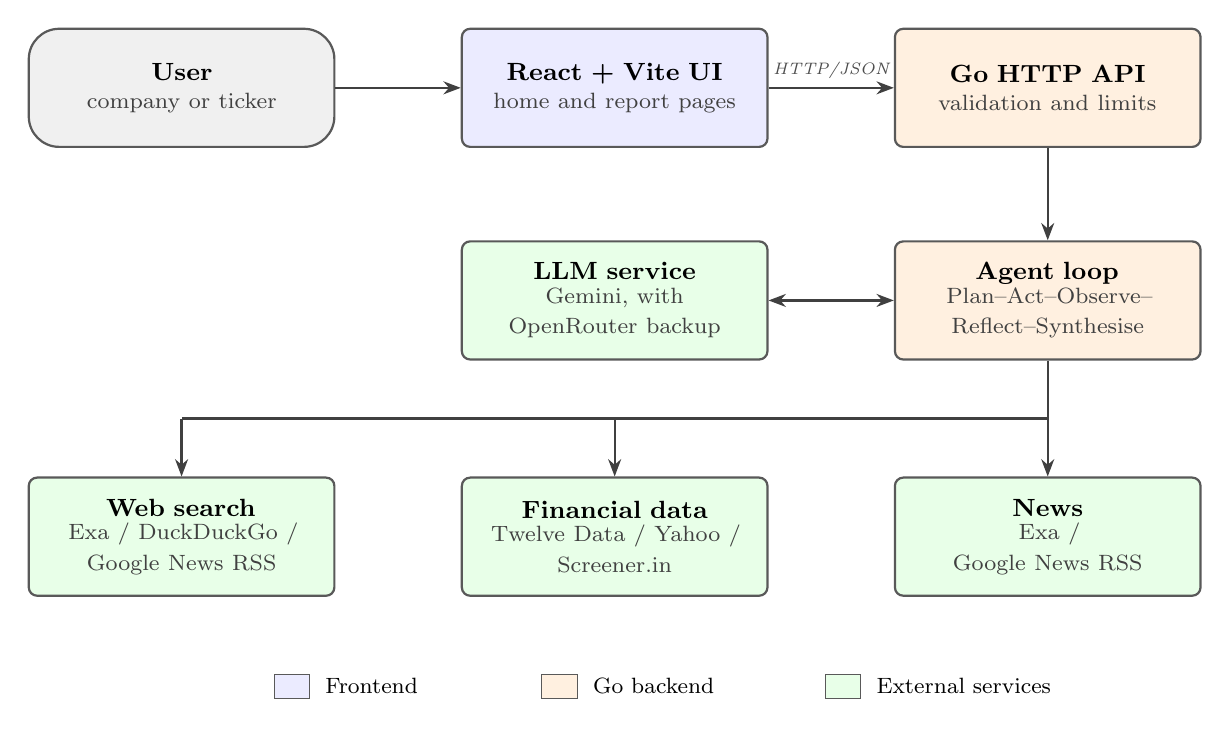
\begin{tikzpicture}[
  font=\small,
  box/.style={draw=black!65,rounded corners=3pt,thick,align=center,text width=3.6cm,minimum height=1.5cm,inner sep=4pt},
  client/.style={box,fill=blue!8},
  server/.style={box,fill=orange!12},
  ext/.style={box,fill=green!9},
  person/.style={box,rounded corners=11pt,fill=black!6},
  sub/.style={font=\footnotesize,text=black!75},
  arr/.style={-{Stealth[length=2.2mm]},thick,black!75},
  line/.style={thick,black!75},
  lab/.style={font=\scriptsize\itshape,text=black!70,inner sep=1pt}]
% row 1: request path
\node[person] (user) at (0,0)    {\textbf{User}\\[-1pt]{\footnotesize\color{black!75}company or ticker}};
\node[client] (ui)   at (5.5,0)  {\textbf{React + Vite UI}\\[-1pt]{\footnotesize\color{black!75}home and report pages}};
\node[server] (api)  at (11.0,0) {\textbf{Go HTTP API}\\[-1pt]{\footnotesize\color{black!75}validation and limits}};
% row 2: orchestration
\node[ext]    (llm)   at (5.5,-2.7)  {\textbf{LLM service}\\[-1pt]{\footnotesize\color{black!75}Gemini, with\\OpenRouter backup}};
\node[server] (agent) at (11.0,-2.7) {\textbf{Agent loop}\\[-1pt]{\footnotesize\color{black!75}Plan--Act--Observe--\\Reflect--Synthesise}};
% row 3: tools
\node[ext] (search) at (0,-5.7)    {\textbf{Web search}\\[-1pt]{\footnotesize\color{black!75}Exa / DuckDuckGo /\\Google News RSS}};
\node[ext] (fin)    at (5.5,-5.7)  {\textbf{Financial data}\\[-1pt]{\footnotesize\color{black!75}Twelve Data / Yahoo /\\Screener.in}};
\node[ext] (news)   at (11.0,-5.7) {\textbf{News}\\[-1pt]{\footnotesize\color{black!75}Exa /\\Google News RSS}};
% arrows
\draw[arr] (user)--(ui);
\draw[arr] (ui)--node[lab,above=3pt,font=\fontsize{6}{7}\itshape\selectfont,inner sep=0pt]{HTTP/JSON}(api);
\draw[arr] (api)--(agent);
\draw[arr,{Stealth[length=2.2mm]}-{Stealth[length=2.2mm]}] (agent)--(llm);
\coordinate (bus) at (11.0,-4.2);
\draw[line] (agent.south)--(bus);
\draw[line] (bus)--(bus -| search);
\draw[arr] (bus -| search)--(search.north);
\draw[arr] (bus -| fin)--(fin.north);
\draw[arr] (bus)--(news.north);
% legend
\node[draw=black!65,fill=blue!8,minimum width=0.45cm,minimum height=0.3cm,label={[font=\footnotesize,xshift=2pt]right:Frontend}] (l1) at (1.4,-7.6) {};
\node[draw=black!65,fill=orange!12,minimum width=0.45cm,minimum height=0.3cm,label={[font=\footnotesize,xshift=2pt]right:Go backend}] (l2) at (4.8,-7.6) {};
\node[draw=black!65,fill=green!9,minimum width=0.45cm,minimum height=0.3cm,label={[font=\footnotesize,xshift=2pt]right:External services}] (l3) at (8.4,-7.6) {};
\end{tikzpicture}
\caption{ResearchAgent architecture (version 1.0).}
\label{fig:architecture}
\end{figure}

A request flows as follows: (1) the user enters a company or ticker on the home page; (2) the report page sends \texttt{POST /api/agent}; (3) the API trims and validates the input and checks the concurrency limit; (4) the agent plans, calls tools, and reflects on what it has; (5) when it has real data it asks the model to write the report, or builds the report itself if the model is unavailable; (6) the API returns the step log and report, which the frontend renders.

\subsection{Agent Orchestration}
The agent (\texttt{internal/agent/agent.go}) runs a loop of at most eight steps, in the spirit of the ReAct pattern~\cite{react-agent} of interleaving reasoning with tool use. On each step the model must reply with one JSON object naming its next action:
\begin{itemize}[leftmargin=*]
\item \textbf{plan} -- a short research plan of three to five steps;
\item \textbf{tool\_call} -- a tool name (\texttt{search}, \texttt{financials}, or \texttt{news}), its arguments, and a reason;
\item \textbf{reflect} -- an assessment of what has been learned so far;
\item \textbf{synthesize} -- a signal that there is enough to write the report.
\end{itemize}
Each tool result is fed back to the model, truncated to 3{,}000 characters (cut on a character boundary so non-ASCII names are not corrupted). If a tool fails, the model is told why, so it can try other parameters or another tool; an empty result is reported as such rather than as success. Unknown tool names and unparseable replies are logged as error steps and the model is asked again. Gemini sometimes wraps its JSON in Markdown fences despite instructions, so the parser strips fences or extracts the first JSON object before decoding.

Figure~\ref{fig:loop} summarises the loop and its exits.
\begin{figure}[H]\centering
\scalebox{0.88}{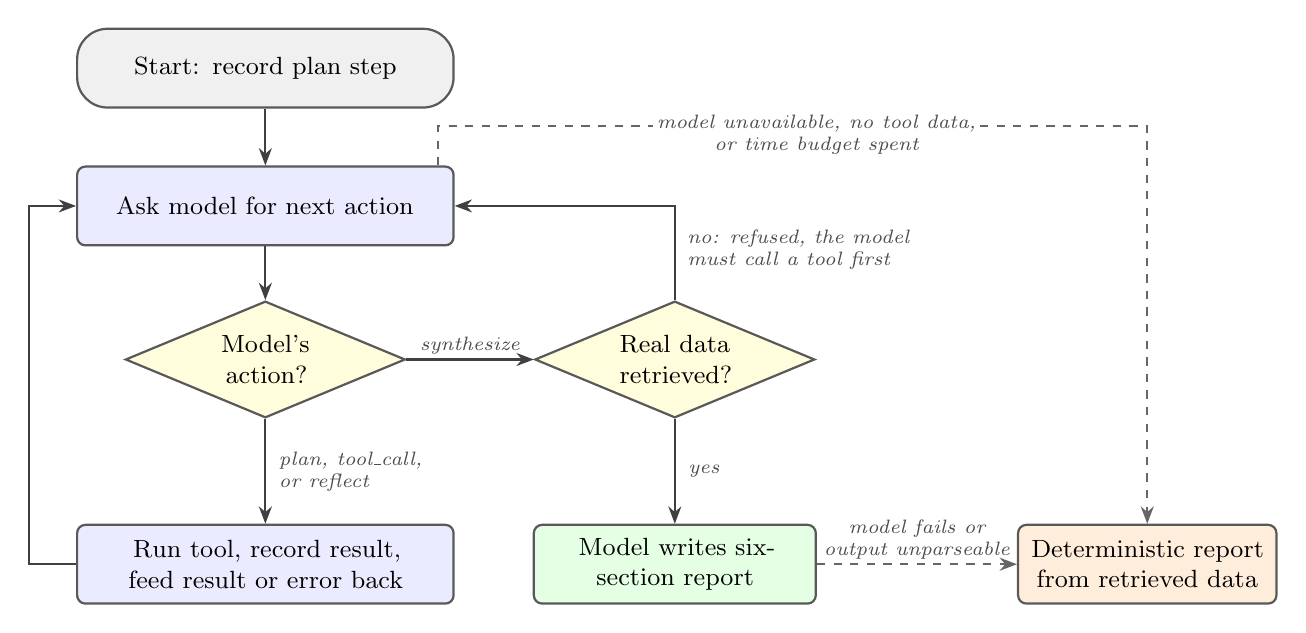
\begin{tikzpicture}[
  font=\small,
  proc/.style={draw=black!65,rounded corners=3pt,thick,align=center,text width=4.5cm,minimum height=1.0cm,fill=blue!8,inner sep=4pt},
  term/.style={proc,rounded corners=11pt,fill=black!6},
  good/.style={proc,text width=3.3cm,fill=green!10},
  fall/.style={proc,text width=3.0cm,fill=orange!14},
  dec/.style={draw=black!65,diamond,aspect=2.4,thick,align=center,fill=yellow!14,inner sep=0pt,text width=2.1cm},
  arr/.style={-{Stealth[length=2.2mm]},thick,black!75},
  darr/.style={-{Stealth[length=2.2mm]},thick,dashed,black!60},
  lab/.style={font=\scriptsize\itshape,text=black!70,inner sep=1.5pt}]
% left column: the research loop
\node[term] (start) at (0,0)    {Start: record plan step};
\node[proc] (ask)   at (0,-1.75) {Ask model for next action};
\node[dec]  (act)   at (0,-3.7) {Model's action?};
\node[proc] (run)   at (0,-6.3) {Run tool, record result, feed result or error back};
% middle column: finishing
\node[dec]  (data)  at (5.2,-3.7) {Real data retrieved?};
\node[good] (write) at (5.2,-6.3) {Model writes six-section report};
% right column: fallback
\node[fall] (fb)    at (11.2,-6.3) {Deterministic report from retrieved data};
% main loop
\draw[arr] (start)--(ask);
\draw[arr] (ask)--(act);
\draw[arr] (act)--node[lab,right=3pt,align=left]{plan, tool\_call,\\or reflect}(run);
\draw[arr] (run.west)--++(-0.6,0)|-(ask.west);
% synthesise path
\draw[arr] (act)--node[lab,above]{synthesize}(data);
\draw[arr] (data)--node[lab,right=3pt]{yes}(write);
% grounding rule: refused, back to the model
\draw[arr] (data.north)|-(ask.east);
\node[lab,anchor=west,align=left] at (5.3,-2.3) {no: refused, the model\\must call a tool first};
% fallback exits (dashed)
\draw[darr] (write)--node[lab,above,align=center]{model fails or\\output unparseable}(fb);
\draw[darr] ([xshift=-6pt]ask.north east)--++(0,0.5)-|(fb.north);
\node[lab,fill=white,align=center] at (7.0,-0.85) {model unavailable, no tool data,\\or time budget spent};
\end{tikzpicture}}
\caption{Agent loop. The dashed path is also taken when the model is unavailable, when no tool returns data, or when the time budget runs out without usable data.}
\label{fig:loop}
\end{figure}

\subsection{Grounding Rules and Deterministic Fallback}
Two rules keep the report tied to retrieved evidence:
\begin{enumerate}[leftmargin=*]
\item \textbf{No report without data.} If the model asks to synthesise before any tool has returned real data, the request is refused and the model is told to call a tool first. The prompts tell the model to use only figures that appear in tool results and to write ``Not available from the retrieved data.'' for any section the results do not support.
\item \textbf{Deterministic fallback.} If the model is unavailable (missing key, quota exhausted, network error), returns a final report that cannot be parsed, or no tool returned data, the agent calls any tools it has not yet used and builds the report directly from their output. The overview, financial snapshot, and news sections are filled from tool data. Competitive landscape, risk factors, and the investment verdict require judgement, so they are explicitly marked as needing the AI model, and the sentiment is left as Neutral (not assessed).
\end{enumerate}
Because of the fallback, the system always returns all six sections, and a missing API key degrades the report instead of breaking it. A configurable time budget (\texttt{RUN\_BUDGET\_SECONDS}, default 90\,s) stops the research phase and writes up whatever has been gathered.

\subsection{Technical Stack}
\begin{table}[H]\centering\small
\begin{tabularx}{\textwidth}{>{\raggedright\arraybackslash}p{3.5cm}X}
\toprule \textbf{Technology} & \textbf{Role in the final system}\\\midrule
Go 1.22 (standard library only) & HTTP API, agent loop, tools; no third-party Go dependencies.\\
React 19, TypeScript 5.7, Vite 6 & Web interface, typed components, and production build.\\
React Router 7 & Home page and \texttt{/report/:company} routing.\\
Tailwind CSS 4 & Responsive, dark styling.\\
Gemini API (2.0 Flash-Lite) & Primary model for planning and report writing.\\
OpenRouter & Optional backup model, tried once if Gemini fails.\\
Twelve Data & Optional preferred source for live prices.\\
Yahoo Finance, Screener.in & Free price and fundamentals sources (Screener.in for Indian tickers).\\
Exa & Optional preferred search and news source.\\
DuckDuckGo HTML, Google News RSS & Free search and news fallbacks.\\
Render & Hosting for the API (web service) and frontend (static site), defined in \texttt{render.yaml}.\\
Git/GitHub & Version control and collaboration.\\
\bottomrule
\end{tabularx}
\caption{Technology stack of version 1.0.}
\label{tab:stack}
\end{table}

\section{Implementation Details}
\subsection{Backend Structure}
The backend in \texttt{analyst-agent-go} is about 2{,}200 lines of Go plus about 970 lines of tests, organised as follows:
\begin{table}[H]\centering\small
\begin{tabularx}{\textwidth}{>{\raggedright\arraybackslash}p{4.2cm}X}
\toprule \textbf{Package} & \textbf{Responsibility}\\\midrule
\texttt{cmd/server} & Entry point: routes, server timeouts, graceful shutdown on SIGTERM.\\
\texttt{internal/httpapi} & Handlers, input validation, CORS, panic recovery, concurrency cap.\\
\texttt{internal/agent} & Research loop, response parsing, deterministic fallback report.\\
\texttt{internal/llm} & Gemini client with OpenRouter backup.\\
\texttt{internal/tools} & Search, news, financials, ticker parsing, Twelve Data and Exa clients.\\
\texttt{internal/types} & Shared data shapes, mirrored in the frontend's \texttt{src/types/index.ts}.\\
\bottomrule
\end{tabularx}
\caption{Backend packages.}
\label{tab:packages}
\end{table}

\subsection{Tools and Fallback Chains}
Every tool returns the same \texttt{ToolResult} shape (tool name, success flag, data, error), so the agent handles all three uniformly. Outbound requests use a 20-second timeout. Each tool tries its sources in order of preference:
\begin{table}[H]\centering\small
\begin{tabularx}{\textwidth}{>{\raggedright\arraybackslash}p{2.2cm}X}
\toprule \textbf{Tool} & \textbf{Source order}\\\midrule
financials & Twelve Data (if keyed) $\rightarrow$ Yahoo Finance $\rightarrow$ Screener.in adds fundamentals for Indian tickers $\rightarrow$ labelled sample data only if \texttt{ALLOW\_SAMPLE\_DATA=1}.\\
news & Exa (if keyed) $\rightarrow$ Google News RSS.\\
search & Exa (if keyed) $\rightarrow$ DuckDuckGo HTML $\rightarrow$ Google News RSS.\\
\bottomrule
\end{tabularx}
\caption{Data-source fallback chains.}
\label{tab:fallbacks}
\end{table}
Several decisions came from tracing real requests through these chains:
\begin{itemize}[leftmargin=*]
\item A ``successful'' response with a zero price counts as a failure, so the chain continues instead of returning an empty quote.
\item For Indian tickers, price and day-change come from Twelve Data or Yahoo, and Screener.in only adds market cap, P/E, and revenue. Earlier, a Twelve Data key made Indian market caps show as N/A.
\item Values a source does not provide (Screener.in's day-change, missing P/E or dividend yield) are left unknown rather than reported as zero.
\item Hard-coded sample figures are off by default and labelled ``Sample data (not live)'' when enabled. Every financial result carries a \texttt{source} field so a reader can tell where the numbers came from.
\end{itemize}

\subsection{Ticker Resolution}
\texttt{internal/tools/ticker.go} turns user input into a symbol:
\begin{table}[H]\centering\small
\begin{tabularx}{\textwidth}{>{\raggedright\arraybackslash}p{5.4cm}X}
\toprule \textbf{Input} & \textbf{Handling}\\\midrule
\texttt{AAPL}, \texttt{aapl}, \texttt{\$AAPL} & Treated as a ticker.\\
\texttt{BRK-B}, \texttt{M\&M.NS}, \texttt{\^{}GSPC}, \texttt{EURUSD=X} & Ticker with punctuation preserved (earlier, \texttt{BRK-B} was mangled to \texttt{BRKB}).\\
\texttt{NASDAQ:AAPL}, \texttt{NSE:TCS} & Exchange prefix removed; \texttt{NSE}/\texttt{BSE} become \texttt{.NS}/\texttt{.BO}.\\
\texttt{Apple Inc.}, \texttt{Infosys} & Built-in table of well-known companies.\\
\texttt{Nvidia Corporation}, \texttt{Zomato Limited} & Looked up through Yahoo Finance symbol search; the result is labelled as a name match.\\
\bottomrule
\end{tabularx}
\caption{Accepted input forms.}
\label{tab:ticker}
\end{table}
A name match is labelled in the result's \texttt{source} (for example, \emph{matched ``Zomato Limited'' to ZOMATO.NS}) because ambiguous names can resolve to the wrong listing. Non-ASCII names are no longer turned into junk tickers, and input made only of symbols is rejected.

\subsection{HTTP API}
\begin{table}[H]\centering\small
\begin{tabularx}{\textwidth}{>{\raggedright\arraybackslash}p{4.4cm}>{\raggedright\arraybackslash}p{3.6cm}X}
\toprule \textbf{Route} & \textbf{Body} & \textbf{Purpose}\\\midrule
\texttt{GET /healthz} & -- & Liveness check; returns \texttt{ok}.\\
\texttt{POST /api/agent} & \texttt{\{"company": ...\}} & Run the full agent.\\
\texttt{POST /api/tools/search} & \texttt{\{"query": ...\}} & Web search only.\\
\texttt{POST /api/tools/financials} & \texttt{\{"ticker": ...\}} & Price and fundamentals only.\\
\texttt{POST /api/tools/news} & \texttt{\{"company": ...\}} & Recent headlines only.\\
\bottomrule
\end{tabularx}
\caption{API routes.}
\label{tab:api}
\end{table}
\texttt{/api/agent} returns an ordered list of messages: one \texttt{step} message per agent step, then a \texttt{report}, then \texttt{done} (or \texttt{error} if the run fails outright). Errors always have the form \texttt{\{"error": "..."\}}: 400 for missing, blank, non-string, or over-100-character input; 405 for the wrong method; 502 when a direct tool call's sources all fail; 503 with \texttt{Retry-After} when the server is busy; and 500 for unexpected errors, which are caught by a recovery middleware.

Production hardening added in the final phase:
\begin{itemize}[leftmargin=*]
\item \textbf{CORS:} \texttt{ALLOWED\_ORIGIN} accepts a comma-separated list and ignores trailing slashes (a trailing slash had silently blocked every browser request). Preflight requests are answered before reaching handlers.
\item \textbf{Concurrency cap:} at most \texttt{MAX\_CONCURRENT\_RUNS} (default 4) agent runs at once, protecting API quotas.
\item \textbf{Timeouts and shutdown:} explicit read, write, and idle timeouts, and a graceful shutdown that lets in-flight runs finish.
\item \textbf{Input hygiene:} newlines and control characters are replaced before input reaches a prompt or a log.
\item \textbf{Key safety:} the Gemini key is sent in a request header rather than the URL, because Go's HTTP errors include the full URL and would otherwise leak the key into logs.
\end{itemize}

\subsection{Frontend}
The frontend in \texttt{analyst-agent-web} is about 630 lines of TypeScript/TSX:
\begin{itemize}[leftmargin=*]
\item \textbf{Home page} (\texttt{src/pages/Home.tsx}): search box with example tickers. It pings \texttt{/healthz} on load so a sleeping free-tier backend starts waking while the user types.
\item \textbf{Report page} (\texttt{src/pages/Report.tsx}): calls the agent, shows a running timer while waiting, then renders the report with the full research log in a collapsible panel. ``Try again'' re-runs the request without reloading the page, and a guard prevents React's development StrictMode from starting a second (paid) agent run.
\item \textbf{Components}: \texttt{ReportCard} renders the six sections and sentiment; \texttt{AgentThinking} and \texttt{ToolCallBadge} (built before the mid-semester evaluation) now display the real step log; \texttt{ErrorBoundary} catches rendering errors.
\item \textbf{API client} (\texttt{src/lib/api.ts}): turns failures into plain-language messages for an unreachable server, a waking backend, a busy server, and timeouts.
\end{itemize}
The layout was checked in a browser at 320, 375, 768, and 1280\,px widths with no horizontal overflow.

\section{Deployment}
\texttt{render.yaml} is a Render Blueprint that creates both services from the repository: a Go web service (\texttt{researchagent-api}) with \texttt{/healthz} as its health check, and a static site (\texttt{researchagent-web}) with a rewrite rule so that refreshing \texttt{/report/AAPL} serves the single-page app instead of a 404. Secrets and cross-service URLs (\texttt{GEMINI\_API\_KEY}, \texttt{ALLOWED\_ORIGIN}, \texttt{VITE\_API\_URL}) are entered in the dashboard and never committed. The top-level README gives the deployment order and a troubleshooting table.

\section{Development Timeline}
\begin{table}[H]\centering\small
\begin{tabularx}{\textwidth}{>{\raggedright\arraybackslash}p{1.5cm}X}
\toprule \textbf{Week} & \textbf{Work completed}\\\midrule
1 & Go module with \texttt{/healthz}; Vite + React + TypeScript project; first shared types.\\
2 & Tool dispatcher and web search tool (DuckDuckGo with Google News RSS fallback); basic Gemini client; frontend types and API client skeleton.\\
3 & News and financials tools; OpenRouter fallback; landing page, Tailwind styling, and routing.\\
4 & Agent loop with deterministic fallback; Twelve Data and Exa as optional sources; agent-activity UI components. (Mid-semester evaluation.)\\
5 & HTTP routes, report page, real API client; financials and agent fixes found by tracing real requests; 25 unit tests and the integration script.\\
6 & Documentation; backend hardening; responsive polish and error messages; ticker edge cases; Render Blueprint; version 1.0.0.\\
\bottomrule
\end{tabularx}
\caption{Week-by-week development.}
\label{tab:timeline}
\end{table}

\chapter{Results and Evaluation}
\label{chap:results}
\section{Final Status Against Objectives}
\begin{table}[H]\centering\small
\begin{tabularx}{\textwidth}{>{\raggedright\arraybackslash}p{3.4cm}X>{\raggedright\arraybackslash}p{2.7cm}}
\toprule \textbf{Objective} & \textbf{Evidence} & \textbf{Status}\\\midrule
Web interface & Home and report pages connected to the real API; production build passes. & Complete\\
Agent loop and tools & Plan/act/reflect/synthesise loop; three tools with fallback chains; agent tests. & Complete\\
Six-section report & Integration check confirms six sections, each with title and content. & Complete\\
Resilience & Source fallbacks, deterministic report, time budget, concurrency cap; tested with fakes. & Complete\\
Deployment & \texttt{render.yaml} Blueprint and documented steps. & Ready; deploy pending\\
Evaluation metrics & Test suite complete; live-data pilot not yet run. & Partially complete\\
\bottomrule
\end{tabularx}
\caption{Final status of each project objective.}
\label{tab:objectives}
\end{table}

\section{Testing}
\subsection{Unit Tests}
The backend has 48 Go test functions (55 including sub-tests). They replace the model, tools, and data sources with fakes, so they run offline and deterministically.
\begin{table}[H]\centering\small
\begin{tabularx}{\textwidth}{>{\raggedright\arraybackslash}p{4.3cm}>{\raggedright\arraybackslash}p{1.3cm}X}
\toprule \textbf{Test file} & \textbf{Tests} & \textbf{What is covered}\\\midrule
\texttt{httpapi/handlers\_test.go} & 16 & Routes, status codes, CORS and origin lists, input validation, concurrency cap, panic recovery.\\
\texttt{agent/agent\_test.go} & 11 & Report shape, grounding rule, fallback paths, JSON parsing, truncation.\\
\texttt{tools/ticker\_test.go} & 11 & Ticker forms, exchange prefixes, name lookup, rejected input.\\
\texttt{tools/financials\_test.go} & 10 & Source ordering, zero-price handling, unknown values, sample-data labelling.\\
\bottomrule
\end{tabularx}
\caption{Unit test coverage.}
\label{tab:unittests}
\end{table}
Tests added in the final week were checked to fail against the old behaviour before the fixes were applied, so they guard against the specific bugs they were written for.

\subsection{Integration Test}
\texttt{scripts/integration\_test.sh} builds and starts the real server and calls it over HTTP the way the browser does. Its 15 checks cover the health route, CORS preflight, rejection of empty, malformed, symbol-only, and over-length input, a readable 502 for an unknown company, and a full agent run that must return steps, a report with six titled sections, a valid sentiment, and a final \texttt{done} message.

\subsection{Verified Results}
All checks were re-run on the final source code:
\begin{table}[H]\centering\small
\begin{tabularx}{\textwidth}{>{\raggedright\arraybackslash}p{5.2cm}X}
\toprule \textbf{Check} & \textbf{Result}\\\midrule
\texttt{go vet ./...} & No issues.\\
\texttt{go test ./...} & 48/48 test functions pass.\\
\texttt{scripts/integration\_test.sh} & 15/15 checks pass; report has 6 sections.\\
\texttt{npm ci \&\& npm run build} & Type-check and production build pass (JS bundle 278\,kB, 88\,kB gzipped).\\
\bottomrule
\end{tabularx}
\caption{Verification results for version 1.0.}
\label{tab:verify}
\end{table}
These runs had no network access to the data sources and no Gemini key, so the integration run exercised the deterministic fallback path end to end. The AI-written path is covered by unit tests with a fake model.

\section{Performance Metrics}
The proposal defined median TTR of at most 60 seconds for a resolved NSE/BSE ticker as the primary metric, with ticker-resolution accuracy, data completeness, fallback trigger rate, and availability as secondary metrics.
\begin{table}[H]\centering\small
\begin{tabularx}{\textwidth}{>{\raggedright\arraybackslash}p{3cm}X>{\raggedright\arraybackslash}p{3.6cm}}
\toprule \textbf{Metric} & \textbf{How it is measured} & \textbf{Status}\\\midrule
Time-to-report & Median time from API receipt to report, over resolved tickers. & Target $\leq 60$\,s; not measured on live data\\
Ticker resolution & Correct mappings divided by tested inputs. & Tested on fixed cases; live accuracy not measured\\
Data completeness & Reports with six source-grounded sections divided by attempts. & Six sections guaranteed by design; grounding not yet reviewed on live runs\\
Fallback trigger rate & Runs using a fallback, by source, divided by total runs. & Not measured\\
Availability & Successful health probes over a stated window. & Not measured (not yet deployed)\\
\bottomrule
\end{tabularx}
\caption{Evaluation metrics and status.}
\label{tab:metrics}
\end{table}
The design bounds the worst case: research stops after 90\,s by default, each outbound data request times out after 20\,s, and model calls time out after 60\,s. Whether the median meets the 60-second target depends on live source and model latency, which the planned pilot of 20--30 large-, mid-, and small-cap NSE/BSE companies would measure. That pilot should log input, resolved ticker, timestamps, tool and fallback events, section completeness, and a manual check of each figure against the returned sources.

\section{Analysis}
The main engineering result is that the system fails safely. Every external dependency---the model, each data source, the hosting platform---can be missing or broken, and the user still gets a clearly labelled report rather than an error page or an invented figure. This came from design choices (the uniform \texttt{ToolResult}, the grounding rule, the deterministic report) and from tracing real requests, which exposed problems the original design did not anticipate: zero prices passing as success, missing values shown as zero, sample data presented as live, the model being told \texttt{null} instead of the tool's error, and tickers with punctuation being mangled.

There are trade-offs. Fallbacks improve reliability but add latency, because each failed source costs up to its timeout before the next is tried. The synchronous API keeps the design simple but means the user sees only a timer, not live steps, until the run ends. Report quality still depends on the model following its instructions; the grounding rule guarantees that real data was retrieved, but only a manual review can confirm that every sentence in an AI-written report is supported by it.

\chapter{Conclusion}
\section{Summary of Work}
ResearchAgent v1.0 is a complete, tested web application that turns a company name or ticker into a six-section research brief. A Go backend runs a Gemini-driven agent loop over three tools with layered free and optional sources, and a React frontend displays the report and the agent's research log. The system handles missing keys, failing sources, ambiguous names, and invalid input without crashing or inventing data. It is covered by 48 unit tests and a 15-check integration test, all passing, and is ready to deploy with a single Render Blueprint.

\section{Key Findings}
\begin{itemize}[leftmargin=*]
\item Separating frontend interaction from backend orchestration gave a clean boundary: the frontend only needed one route and one message format.
\item A uniform result shape for every tool made fallbacks, error reporting, and testing much simpler.
\item Grounding has to be enforced in code, not only in prompts: the ``no report without data'' rule and the deterministic report stop the model from writing from memory.
\item Treating ``no value'' as unknown rather than zero, and labelling where every figure came from, matters as much as fetching the figure.
\item Injecting the model and tools as replaceable functions let the whole agent be tested offline.
\item Credible evaluation needs both operational metrics and a factual review of reports; speed and six filled headings are not enough.
\end{itemize}

\section{Limitations}
\begin{itemize}[leftmargin=*]
\item \texttt{/api/agent} is synchronous, so the research log appears only after the run finishes.
\item DuckDuckGo and Screener.in are scraped and can break when those sites change their markup.
\item Name-based lookup can pick the wrong listing for ambiguous names; the result is labelled, and typing the ticker avoids the guess.
\item Abuse protection is a global cap on concurrent runs, not per-user rate limiting or authentication.
\item On Render's free plan the backend sleeps when idle, so the first request can take about a minute longer.
\item Live-data behaviour, the deployed services, and TTR have not yet been measured.
\end{itemize}

\section{Future Work}
\begin{enumerate}[leftmargin=*]
\item Deploy both services, tag \texttt{v1.0.0}, and run the 20--30 company pilot to report actual TTR, resolution accuracy, completeness, fallback rate, and availability.
\item Stream agent steps to the browser (server-sent events) so users can watch the research live.
\item Attach source links to individual claims in the report, so each figure can be traced to the result it came from.
\item Add per-user rate limiting and short-lived caching of tool results for repeated companies.
\item Add continuous integration that runs \texttt{go vet}, the Go tests, the integration script, and the frontend build on every push.
\item Replace scraped sources with official APIs where free tiers allow.
\end{enumerate}

\section{Final Remarks}
ResearchAgent applies established engineering practice to an information-access problem: modular architecture, explicit tool orchestration, layered fallbacks, typed interfaces, and automated tests. Its value lies in the traceability and honesty of its reports---saying ``not available'' when evidence is missing---rather than in fluent output alone. The remaining step is to measure it on live data and confirm the performance target that the design is built to meet.

\begin{thebibliography}{99}
\bibitem{proposal} A. Khanduja, G. Sharma, and V. Choudhary, \textit{ResearchAgent: An Autonomous AI Agent for Stock and Company Research}, Project Proposal for UCS503P, Thapar Institute of Engineering and Technology, August 25, 2026.
\bibitem{react} Meta Open Source, \textit{React Documentation}. Available: \url{https://react.dev/}. Accessed November 2026.
\bibitem{vite} Vite Contributors, \textit{Vite Documentation}. Available: \url{https://vite.dev/}. Accessed November 2026.
\bibitem{ts} Microsoft, \textit{TypeScript Documentation}. Available: \url{https://www.typescriptlang.org/docs/}. Accessed November 2026.
\bibitem{tailwind} Tailwind Labs, \textit{Tailwind CSS Documentation}. Available: \url{https://tailwindcss.com/docs}. Accessed November 2026.
\bibitem{go} The Go Authors, \textit{Go Documentation}. Available: \url{https://go.dev/doc/}. Accessed November 2026.
\bibitem{gemini} Google, \textit{Gemini API Documentation}. Available: \url{https://ai.google.dev/gemini-api/docs}. Accessed November 2026.
\bibitem{openrouter} OpenRouter, \textit{API Documentation}. Available: \url{https://openrouter.ai/docs}. Accessed November 2026.
\bibitem{twelvedata} Twelve Data, \textit{API Documentation}. Available: \url{https://twelvedata.com/docs}. Accessed November 2026.
\bibitem{exa} Exa, \textit{API Documentation}. Available: \url{https://docs.exa.ai/}. Accessed November 2026.
\bibitem{render} Render, \textit{Documentation}. Available: \url{https://render.com/docs}. Accessed November 2026.
\bibitem{react-agent} S. Yao \textit{et al.}, ``ReAct: Synergizing Reasoning and Acting in Language Models,'' in \textit{Proc. ICLR}, 2023.
\end{thebibliography}
\end{document}